\documentclass{article}
\usepackage{graphicx} 
\usepackage{amsmath}
\usepackage{kotex}
\usepackage{moresize}
\setlength{\linewidth}{2mm}
\title{Quantum Theory of Materials}
\author{권정우}
\date{January 2025}

\begin{document}

\maketitle
\section*{Introduction}
These notes are concise reformulation of the knowledge I gained regarding quantum mechanical theory of materials during my service at Republic of Korea Army (Imsil, Jeonbuk Province. 12.26.2023-06.25.2025). They were written over the period of 01.26.2025-04.30.2025\\
\\
\textit{References}\\
\\
Ashcroft, N. and Mermin, N. D., \textit{Solid State Physics} (Cengage Learning, Boston, 1976).\\
\\
Girvin S. M. and Yang K., \textit{Modern Condensed Matter Physics} (Cambridge University Press, Cambridge, 2019).\\
\\
Marder, M. P., \textit{Condensed Matter Physics} (Wiley, New Jersey, 2016).\\
\\
Cohen, M. L. and Louie, S. G., \textit{Fundamentals of Condensed Matter Physics} (Cambridge University Press, Cambridge, 2016).\\
\\
Martin, R. M., \textit{Electronic Structure: Basic Theory and Practical Methods} (Cambridge University Press, Cambridge, 2020).\\
\\
Giustino, F., \textit{Materials Modelling Using Density Functional Theory: Properties and Predictions} (Oxford University Press, Oxford, 2014).\\
\\
Sakurai, J. J. and Napolitano, J., \textit{Modern Quantum Mechanics} (Cambridge University Press, Cambridge, 2016)\\
\\
The 3rd APCTP-KIAS Electronic Structure Calculations Winter School (18-20 January 2023). http://events.kias.re.kr/h/KA2023/?pageNo=4947\\
\section*{Contents}
\begin{enumerate}
	\item Construction of the Hamiltonian
	\item The Electronic Band Structure
	      \begin{enumerate}
		      \item Bloch Theorem and Brillouin Zone
		      \item Free Electron Gas
		      \item Nearly Free Electron Model
		      \item Tight Binding Model
		      \item Semi-Classical Equation
	      \end{enumerate}
	\item Hartree-Fock Approximation
	\item Density Functional Theory
	      \begin{enumerate}
		      \item Hohenberg Kohn Functional
		      \item Kohn Sham Equation
		      \item Functional form of $E_{XC}[n]$
	      \end{enumerate}
	\item Quasiparticles
	      \begin{enumerate}
		      \item Landau Fermi Liquid Theory
		      \item Quasielectron
		      \item Phonon
	      \end{enumerate}
\end{enumerate}
\section*{Construction of the Hamiltonian}
The Hamiltonian, $H$ contains all information of the system in interest. It is well known from non-relativistic quantum theory that $H$ determines the time evolution of the state $|\psi\rangle$ via the Schrodinger equation
\begin{equation}
	i\hbar\partial_{t}|\psi\rangle=H|\psi\rangle
\end{equation}
We are more interested in the time-independent aspect of things so taking the eigenstate of $H$ yields
\begin{equation}
	H|\phi\rangle=E|\phi\rangle
\end{equation}
$|\phi\rangle$ is now a stationary state with the following time-dependence
\begin{equation}
	|\phi (t)\rangle=|\phi\rangle e^{-iEt/\hbar}
\end{equation}
We will now denote stationary state $|\psi\rangle$ since no differentiation of $|\psi\rangle$ and $|\phi\rangle$ will be required.\\
A condensed matter system(mostly solid for my primary interest) is composed of huge($\sim10^{24}$) number of constituents; electrons, protons, neutrons etc. Since condensation requires our theory to naturally be a 'low-energy' theory we effectively take into account only the valence electron and core(nucleus and inert electrons) degrees of freedom. \\
Our Hamiltonian should take into account interaction between these components plus the external potential.
\begin{equation}
	H=T_{c}+T_{e}+V_{cc}+V_{ce}+V_{ee}+V_{ext}
\end{equation}
$T$ denotes kinetic energy and $V$, the two-body Coulombic interaction among core and electrons. Expressing core and valence electron variables as upper and lowercase letters respectively and ignoring external potential $V_{ext}$ for the moment, the full Hamiltonian writes
\begin{multline}
	H=\sum_{I}\frac{P_{I}^{2}}{2M_{I}}+\sum_{i}\frac{p_{i}^{2}}{2m_{i}}+\frac{1}{2}\sum_{I\neq J}\frac{e^{2}}{4\pi\epsilon_{0}}\frac{Z_{I}Z_{J}}{|R_{I}-R_{J}|}+\\
	\frac{1}{2}\sum_{i\neq j}\frac{e^{2}}{4\pi\epsilon_{0}}\frac{z_{i}z_{j}}{|r_{i}-r_{j}|}-\sum_{i,I}\frac{e^{2}}{4\pi\epsilon_{0}}\frac{Z_{I}}{|R_{I}-r_{i}|}
\end{multline}
$H$, though 'exact' in our schematic, contains high complexity considering the summation index over all electron and core coordinates. Seeking exact solution to this Hamiltonian is pure non-sense, which is why further approximation scheme is needed for simplification.\\
Also, for the sake of notational simplicity, we use the Hartree units, where we measure distances in Bohr's radius $a_0=\frac{4\pi\epsilon_0\hbar^2}{e^2m_e}=1$ and measure energy in Hartree units $E_{Ha}=\frac{e^2}{4\pi\epsilon_0a_0}=1$. Also, we exploit the operator relation $\mathbf{p}\to i\nabla$\\
In the Born-Oppenheimer adiabatic approximation or simply the clamped nuclei approximation we recall $T_{c}<<T_{e}$ since cores are much massive than electrons. Higher core mass ($Z_{I}$) only strengthens this relation by Coulomb interaction. We take $T_{c}$ as a small constant $\epsilon$  independent of other parameters and simply take $H-\epsilon$ as our new $H$
\begin{multline}
	H=\sum_{i}-\frac{\nabla_i^{2}}{2}+\frac{1}{2}\sum_{I\neq J}\frac{Z_{I}Z_{J}}{|R_{I}-R_{J}|}+
	\frac{1}{2}\sum_{i\neq j}\frac{1}{|r_{i}-r_{j}|}-\sum_{i,I}\frac{Z_{I}}{|R_{I}-r_{i}|}
\end{multline}
By the same token, $V_{cc}$ can be taken as an independent constant since $\partial_{t} R_{I}\to0$. Repeating the procedure, $H-V_{cc}$ is our new effective Hamiltonian.
\begin{equation}
	H=\sum_{i}-\frac{\nabla_i^{2}}{2}+\frac{1}{2}\sum_{i\neq j}\frac{1}{|r_{i}-r_{j}|}-\sum_{i,I}\frac{Z_{I}}{|R_{I}-r_{i}|}\label{themasterhamiltonian}
\end{equation}
Though our last approximation is valid, we will relax this approximation in the future discussion of phonon(collective vibration modes of lattice).\\
Another approximation that reduces complexity is the "Independent Electron Approximation". We drop the electron-electron interaction term \\
$\frac{1}{2}\sum_{i\neq j}\frac{1}{|r_{i}-r_{j}|}$. This bold approximation fits well for surprisingly large class of materials and will be justified by Landau's Fermi liquid theory.
\begin{equation}
	H=\sum_{i}-\frac{\nabla_i^{2}}{2}-\sum_{i,I}\frac{Z_{I}}{|R_{I}-r_{i}|}
\end{equation}
Taking the $i$ summation outside,
\begin{equation}
	H=\sum_{i}\left(-\frac{\nabla_i^{2}}{2}-\sum_{I}\frac{Z_{I}}{|R_{I}-r_{i}|}\right)
\end{equation}
Terms inside the parentheses is the Hamiltonian which a single electron experiences in the core-crystal environment. Denoting this Hamiltonian $h_{i}$,
\begin{equation}
	H=\sum_{i}h_{i}
\end{equation}
We have succeeded in reducing the Hamiltonian into a sum of Hamiltonian each individual electron experiences. Our initial interest is to survey this $h_{i}$
\section*{The Electronic Band Structure}
\subsection*{Bloch Theorem and Brillouin Zone}
Focusing on the independent electron's journey through our prearranged Hamiltonian,
\begin{equation}
	h=-\frac{\nabla^{2}}{2}+V\label{singleelctronHamiltonian}
\end{equation}
Most solids form crystalline structures. This requires further symmetry on $h$. Since $\mathbf{R}_{I}$s contributing to $V$ would have periodic lattice structures,
\begin{equation}
	V(\mathbf{r})=V(\mathbf{r}+\mathbf{R})=V(\mathbf{r}+n\mathbf{R})\label{BvK}
\end{equation}
$\mathbf{R}$ is the primitive lattice translation vector. This periodic boundary condition \eqref{BvK} is also known as the Born-von-Karman boundary condition.\\
$-\frac{\nabla^{2}}{2}$ is dependent only on electron coordinate, allowing the translation operator $T_{\mathbf{R}}$ to commute with $h$
\begin{equation}
	[h,T_{\mathbf{R}}]=0\label{13}
\end{equation}
Further inspection of $T_\mathbf{R}$ is bound to yield good quantum numbers for describing $h$ eigenstate.\\
From the interpretation of momentum as generator of translation, $T_\mathbf{R}$ operates on $|\psi\rangle$ as $T_{\mathbf{R}}\to e^{i\mathbf{p}\cdot\mathbf{R}/\hbar}$. Since $\mathbf{p}/\hbar$ takes the dimension of 1/length, $\mathbf{p}/\hbar$ can be written as a usual wave vector $\mathbf{k}$. So $T_{\mathbf{R}}\to e^{i\mathbf{k}\cdot\mathbf{R}}$.
But this $\mathbf{k}$ is not our usual wave vector since translation takes only discrete values($n\mathbf{R}$) due to lattice geometry. We can induce that discrete translational symmetry will lead to discretely conserved quantity $\hbar\mathbf{k}$, which has the dimension of momentum. We indeed call this quantity the 'crystal momentum' of the lattice.\\
Let's return to the basic theorem that $h$ and $T_{\mathbf{R}}$ will have simultaneous eigenstates from eq. \eqref{13}
\begin{equation}
	h|\psi\rangle=E|\psi\rangle
\end{equation}
\begin{equation}
	T_{\mathbf{R}}|\psi\rangle=c(\mathbf{R})|\psi\rangle
\end{equation}
$T_{\mathbf{R}}$ has the following group properties.
\begin{equation}
	T_{\mathbf{R}}T_{\mathbf{R'}}=T_{\mathbf{R+R'}}
\end{equation}
\begin{equation}
	T_{\mathbf{-R}}=T_{\mathbf{R}}^{-1}
\end{equation}
\begin{equation}
	T_\mathbf{R}T_{\mathbf{R}}^{\dagger}=\mathbf{1}\label{unitarity}
\end{equation}
Taking $\mathbf{a_{1}},\mathbf{a_{2}},\mathbf{a_{3}}$ as primitive translation vector of the lattice $\mathbf{R}$ and considering the above properties,
\begin{equation} c(\mathbf{R})=c(n_{1}\mathbf{a}_{1}+n_{2}\mathbf{a}_{2}+n_{3}\mathbf{a_{3}})=c(\mathbf{a_{1}})^{n_{1}}c(\mathbf{a_{2}})^{n_{2}}c(\mathbf{a_{3}})^{n_{3}}
\end{equation}
From the definition of reciprocal lattice $\mathbf{G}$,
\begin{equation}
	\mathbf{G}=h_{1}\mathbf{b}_{1}+h_{2}\mathbf{b}_{2}+h_{3}\mathbf{b}_{3}
\end{equation}
\begin{equation}
	\mathbf{a}_{i}\cdot\mathbf{b}_{j}=2\pi\delta_{ij}
\end{equation}
and together with relations \eqref{BvK}, \eqref{unitarity}  we conclude
\begin{equation}
	c(\mathbf{R})=e^{i\mathbf{k\cdot R}}
\end{equation}
where $\mathbf{k}=\mathbf{G}/n$. This condition comes from the Born-von-Karman boundary condition requiring
\begin{equation}
	c^{n}(\mathbf{R})=1
\end{equation}
We know have our final conclusion,
\begin{equation}
	T_{\mathbf{R}}\psi(\mathbf{r})=\psi(\mathbf{r+R})=e^{i\mathbf{k}\cdot\mathbf{R}}\psi(\mathbf{r})\label{bloch1}
\end{equation}
or equivalently
\begin{equation}
	\psi(\mathbf{r})=e^{i\mathbf{k}\cdot\mathbf{r}}u(\mathbf{r}),\hspace{1cm}u(\mathbf{r})=u(\mathbf{r}+\mathbf{R})\label{bloch2}
\end{equation}
Equations \eqref{bloch1}, \eqref{bloch2} are known as the Bloch theorem and is fundamental in our study of solids. It tell us that periodic Hamiltonian need only be solved in one unit cell; adjacent unit cell has $|\psi\rangle$ differing only by a factor of $e^{i\mathbf{k}\cdot\mathbf{R}}$.\\
Another deduction is that an electron experiencing a periodic crystal Hamiltonian need not scatter randomly, like in Drude's theory of electrical conductivity.\\
$|\psi\rangle$'s coherence allows it to be a periodic modulation $u(\mathbf{r})$ to a plane wave $e^{i\mathbf{k}\cdot\mathbf{r}}$. A perfect periodic crystal will have infinite conductivity.\\
Discrete values of $\mathbf{R}$ requires $\mathbf{k}$ to be inside a certain unit cell of the reciprocal lattice $\mathbf{G}$, more specifically,
\begin{equation}
	\mathbf{k}=\frac{\alpha_{1}}{2\pi}\mathbf{b}_{1}+\frac{\alpha_{2}}{2\pi}\mathbf{b_{2}}+\frac{\alpha_{3}}{2\pi}\mathbf{b}_{3}(0\leq\alpha\leq2\pi)\label{kG}
\end{equation}
This is equivalent to saying $\mathbf{k}$ is restricted in the first Brillouin Zone, the Wigner Seitz Cell of the reciprocal lattice.\\
But the restriction $0\leq\alpha\leq2\pi$ isn't as necessary, rsulting in ambiguity of $c(\mathbf{R})$. The ambiguity comes from the redundant description of states from the following transformation


\begin{equation}
	\mathbf{k}\to\mathbf{k+n\mathbf{G}}
\end{equation}
This doesn't change the physics of $\psi(\mathbf{r})$, since it only works as multiplying a trivial phase $e^{i\cdot2\pi}$. $\mathbf{k}$ is said to be in the $n$th Brillouin Zone when
\begin{equation}
	2(n-1)\pi\leq\alpha_{i}\leq2n\pi
\end{equation}
$n$ is defined as the Band Index, number of translations in $\mathbf{G}$ required to put $\mathbf{k}$ in the first Brillouin Zone. (This definition of Brillouin zone works only in one dimension, they are originally defined as Wigner-Seitz cells of reciprocal lattice)\\
$n$ and $\mathbf{k}$ are good quantum numbers for describing 'bloch eigenstates', eigenstates of periodic Hamiltonian.\\
From \eqref{bloch1}, $u(\mathbf{r})$'s periodicity can be exploited from periodic functions have discrete Fourier sum.
\begin{equation}
	\psi(x)=e^{i\mathbf{k}\cdot\mathbf{r}}u(\mathbf{r})=e^{i\mathbf{k}\cdot\mathbf{r}}\sum_{\mathbf{G}}b_{\mathbf{k}}(\mathbf{G})e^{i\mathbf{G}\cdot\mathbf{r}}\label{bloch3}
\end{equation}
Substituting this result in the eigenvalue equation for the single electron hamiltonian $h$ in \eqref{singleelctronHamiltonian}, we acquire
\begin{equation}
	\left(\frac{1}{2m_{e}}\left(\mathbf{\hat{p}}^{2}+2\hbar\mathbf{k}\mathbf{\hat{p}}+\hbar^{2}\mathbf{k}^{2}\right)\right)u_{n,\mathbf{k}}(\mathbf{r})=\epsilon_{n}(\mathbf{k})u_{n,\mathbf{k}}(\mathbf{r})\label{eigenvalueeqwithbandstructure}.
\end{equation}
$\epsilon_{n}(\mathbf{k})$, the eigenvalue of this equation is the electronic band structure. It takes the 'good' quantum numbers $n$ and $\mathbf{k}$ as index.\\
In discussing band structure, information in $\mathbf{r}$ is rather insignificant to our interest. Our primary interest is in the momentum space($\mathbf{p}/\hbar$ to be exact), due to the fact that discrete translational symmetry requires to take $\mathbf{k}$ as the quantum number(state index). In quantum mechanics, $\mathbf{r}$ space representation and $\mathbf{p}$ space representation is related by Fourier transform.
\begin{equation}
	\langle\mathbf{r}|\mathbf{p}\rangle=\frac{1}{(2\pi\hbar)^{3/2}}e^{i\mathbf{k}\cdot\mathbf{r}}
\end{equation}
$\mathbf{r}$ space representation relates to the real lattice, $\mathbf{p}$($\mathbf{p}/\hbar$) space representation relates to  the Fourier transform of the real lattice, the reciprocal lattice.($\mathbf{k}$ lattice if considering $\hbar$). We will later see the representation of electronic states in $\mathbf{k}$ space and how the geometry of Fermi Surface in $\mathbf{k}$ space effect solid properties.\\
Equation \eqref{eigenvalueeqwithbandstructure} also tells us that band structure $\epsilon_{n}(\mathbf{k})$ has equivalent symmetry as $\mathbf{R}$, the crystal lattice.\\
Consider a unitary symmetry operator $\theta$ that transforms as  $\mathbf{r}\to\theta\mathbf{r}$, such as the crystal point group. Since unitarity assures $\langle\mathbf{\hat{p'}}|\mathbf{\hat{p'}}\rangle=\langle\mathbf{\hat{p}}|\mathbf{\hat{p}}\rangle$, $\langle\mathbf{\hat{k'}}|\mathbf{\hat{k'}}\rangle=\langle\mathbf{\hat{k}}|\mathbf{\hat{k}}\rangle$, $\langle\mathbf{\hat{k'}}|\mathbf{\hat{p'}}\rangle=\langle\mathbf{\hat{k}}|\mathbf{\hat{p}}\rangle$
\begin{equation}
	\left(\frac{1}{2m_{e}}\left(\mathbf{\hat{p}}^{2}+2\hbar\mathbf{k}\mathbf{\hat{p}}+\hbar^{2}\mathbf{k}^{2}\right)\right)u_{n,\mathbf{k}}(\theta\mathbf{r})=\epsilon_{n}(\mathbf{k'})u_{n,\mathbf{k}}(\theta\mathbf{r})\label{eigenfunctiontheta}.
\end{equation}
So, the same $\theta$ satisfies
\begin{equation}
	\epsilon_{n}(\mathbf{k}')=\epsilon_{n}(\theta\mathbf{k})=\epsilon_{n}(\mathbf{k})
\end{equation}
Thus, $\epsilon_{n}(\mathbf{k})$ has the symmetry of $\mathbf{R}$. Releasing the requirement of $\mathbf{k}$ being in the first Brillouin Zone, $\theta$ may include the crystal space group.(Symmetry considerations including lattice translation.)\\
Time Reversal operation, which mathematically is an anti-unitary complex conjugation relates $\psi(\mathbf{r})$ with spin degree of freedom. $\epsilon_{n}(\mathbf{k})$, in turn acquires the Kramer's degeneracy,
\begin{equation}
	\epsilon_{n}(\uparrow\mathbf{k})=\epsilon_{n}(\downarrow-\mathbf{k})
\end{equation}
\subsection*{Free Electron Gas}
Before giving further detail to our periodic potential $V(\mathbf{r})$, we will discuss the $V(\mathbf{r})=0$ case, also known as the free electron model. The free electron model will serve as a background to which $V(\mathbf{r})$ will perturb. The electron gas are free, non-interacting fermions subject to the big box normalization condition
$$V=\begin{cases}
		0\qquad 0<x,y,z<L \\
		\infty \qquad otherwise
	\end{cases}$$
From solving elementary time-independent Schrodinger equation we have the stationary state $\psi(\mathbf{r})$
$$\psi(\mathbf{r})=\frac{e^{i \mathbf{k}\cdot\mathbf{r}}}{\sqrt{\mathcal{V}}}$$
$\mathcal{V}$ is the volume of the 'big box', $\mathcal{V}=L^3$. This stationary state is a plane wave state, with quantization condition
$$k_{i}=\frac{2n\pi}{L}\quad (n_i\in \mathcal{N})$$
We later see that $\mathbf{k}$ has equal footings as $\mathbf{k}$ that indexes Bloch state.\\
From the quantization rule, free electron states can be denoted in the $\mathbf{k}$ space 'grid' with grid volume $\Omega=8\pi^{3}/V$. Likewise in the previous discussion of Bloch theorem, $\mathbf{k}$ space will be more suitable in showing momentum information.\\
The energy eigenvalue of this $\mathbf{k}$ state is $\hbar^2\mathbf{k}^2/2m$, which we will denote as $E_\mathbf{k}^0$ from now on. This eigenvalue is proportional to the squared distance from the origin in $\mathbf{k}$ space. There are as many states as there are free electrons, occupying this space starting from grid closest to the origin. (2 states each grid when considering spin degeneracy). If the grid volume $\Omega$ is small enough and the number of states big enough, states will occupy the $\mathbf{k}$ space on the positive octant of a sphere.\\
We define $\mathbf{k}$ that differentiates occupied from occupied state, the 'radius' of occupation as the Fermi wave vector $\mathbf{k}_F$. The surface that $\mathbf{k}_F$ lies on is defined as the Fermi surface. (Spherical shell in the free electron case) Electrons on the Fermi surface is significant in determining the property of materials. \\
Many Fermi-quantities are defined. Fermi momentum $\mathbf{p}_F=\hbar\mathbf{k}_F$, Fermi velocity $\mathbf{v}_F=\mathbf{p}_F/m$, Fermi energy $E_F=\mathbf{p}_F^2/2m$, Fermi temperature $T_F=E_F/k_B$, Fermi Pressure $2E_F/3V$. Fermi pressure accounts to some degree, the 'rigidity' of solids, even though the interactive forces between electrons weren't considered, only their fermionic nature.\\
The number of states in a certain energy range $(E,E+dE)$ (in many case of interest, $E\sim E_F$) will be important. Density of states $D(E)$ is defined as that number.
$$\int_E^{E+dE}D(E)dE=n(E), \quad D(E)=\frac{\partial n(E)}{\partial E}$$
We can compute $D(E)$ in complete form in the free electron case,
$$\int_0^{E_F} D(E)dE=N$$
Counting $D(E)$ in 3D free electron gas is fairly simple, considering the geometry in $k$-space,
$$n_x^2+n_y^2+n_z^2=\frac{2mL^2}{\hbar^2\pi^2} E$$
With a conversion to $n$-space with $k_i=\frac{2n_i\pi}{L}$, $n(E)$ is a 'volume' in positive octant of occupation in $n$-space(each grid takes a volume of $1^3$.
$$n(E)=\frac{1}{8}\frac{4\pi}{3}(\frac{2mL^2}{\hbar^2\pi^2})^\frac{3}{2}=\frac{\mathcal{V}}{6\pi^2}\frac{2m}{\hbar^2}^\frac{3}{2}E^\frac{3}{2}$$
If we want to consider spin-degeneracy just multiply with factor 2.(This degeneracy is broken with external magnetic field). From $D(E)=\frac{\partial n(E)}{\partial E}$,
$$D(E)/\mathcal{V}=\frac{1}{2}\frac{2m}{\hbar^2}^{\frac{3}{2}}\sqrt{E}$$
$D(E)$ goes like $E^{\frac{1}{2}}$ in 3D free electron gas. The free electron gas density of states may be generalized to d-dimensions,
$$D^d(E)=\frac{\mathcal{V}}{(2\pi)^d}\frac{(2\pi)^\frac{d}{2}}{\Gamma(\frac{d}{2})}\frac{2m}{\hbar}^{\frac{d}{2}}E^{\frac{d}{2}-1}$$
Notice the density of states being independent of $E$ in 2D, decreasing in 1D.
\subsection*{Nearly Free Electron Model}
In the Nearly Free Electron Model(NFEM), we weakly turn on the perturbation $V(\mathbf{r})$ which has the periodicity of real lattice $\mathbf{R}$. Since periodicity information that $V$ has will be Fourier transformed in to $\mathbf{k}$ space, perturbation will be related to reciprocal lattice $\mathbf{G}$.\\
Consider \eqref{13} in the form of $(h-E)|\psi\rangle=0$. $|\psi\rangle$ will be periodic in $\mathbf{r}$, its Fourier transform will contain infinite but discrete sum
\begin{equation}
	|\psi\rangle=\frac{1}{\sqrt{\mathcal{V}}}\sum_{\mathbf{k}}\psi(\mathbf{k})e^{i\mathbf{k\cdot\mathbf{r}}}\label{ft of psi}
\end{equation}
$V(\mathbf{r})$'s Fourier transform also has discrete sum but with its periodicity specified in $\mathbf{R}$, its Fourier component will contain reciprocal lattice vector $\mathbf{G}$.
\begin{equation}
	V(\mathbf{r})=\sum_{\mathbf{G}}V(\mathbf{G})e^{i\mathbf{G}\cdot\mathbf{r}}\label{ft of V}
\end{equation}
Substituting the relations \eqref{ft of psi} and \eqref{ft of V} into $(h-E)|\psi\rangle=0$
$$\frac{1}{\sqrt{\mathcal{V}}}\sum_{\mathbf{k}}\left[E_{\mathbf{k}}^{0}-E+V(\mathbf{r})\right]\psi(\mathbf{k})e^{i\mathbf{k}\cdot\mathbf{r}}=$$
$$\frac{1}{\sqrt{\mathcal{V}}}\sum_{\mathbf{k}}\left[(E_{\mathbf{k}}^{0}-E)e^{i\mathbf{k}\cdot\mathbf{r}}+\sum_{\mathbf{G}}e^{i(\mathbf{G}+\mathbf{k})\cdot\mathbf{r}}V(\mathbf{G})\right]\psi(\mathbf{k})=0$$
Operating $\int d\mathbf{r}e^{-i\mathbf{k'}\cdot\mathbf{r}}$ on both sides and using the relation $\int d\mathbf{r}e^{i\mathbf{k}\cdot\mathbf{r}}=2\pi\delta(\mathbf{k})$
$$\frac{1}{\sqrt{\mathcal{V}}}\int d\mathbf{r}\left(\sum_{\mathbf{k}}\left[(E_{\mathbf{k}}^{0}-E)e^{i(\mathbf{k}-\mathbf{k'})\cdot\mathbf{r}}+\sum_{\mathbf{G}}e^{i(\mathbf{G}+\mathbf{k}-\mathbf{k'})\cdot\mathbf{r}}V(\mathbf{G})\right]\right)\psi(\mathbf{k})=0$$
$$\frac{1}{\sqrt{\mathcal{V}}}\sum_{\mathbf{k}}\left((E_{\mathbf{k}}^{0}-E)\delta_{\mathbf{k'}\mathbf{k}}+\sum_{G}V(\mathbf{G})\delta_{\mathbf{k+G},\mathbf{k'}}\right)\psi(\mathbf{k})=$$
$$\frac{1}{\sqrt{\mathcal{V}}}\sum_{\mathbf{k}}\left((E_{\mathbf{k}}^{0}-E)\psi(\mathbf{k})+\sum_{G}V(\mathbf{G})\psi(\mathbf{k+G})\right)=0$$
We replace the Fourier component of $\psi(\mathbf{r})$ to $|\mathbf{k}\rangle$  and $V(\mathbf{r})$ to $V_{\mathbf{G}}$, resulting in
\begin{equation}
	\sum_{\mathbf{k}}\left((E_{\mathbf{k}}^{0}-E)|\mathbf{k}\rangle+\sum_{G}V_{\mathbf{G}}|\mathbf{k+G}\rangle\right)=0 \label{CentralEquation}
\end{equation}
This Fourier transformed version of the time-independent Schrodinger equation is known as the central equation. Truncation of the central equation upto reasonable terms may yield accurate and computationally effective result.
The Original one-body Hamiltonian $h$ is restored in Dirac notation in the following form.
\begin{equation}
	h=\sum_{\mathbf{k}}\left(|\mathbf{k}\rangle E_{\mathbf{k}}^{0}\langle\mathbf{k}|+\sum_{\mathbf{G}}|\mathbf{k}\rangle V_{\mathbf{G}}\langle\mathbf{k+G}|\right)\label{hindirac}
\end{equation}
In this form, it is easy to see $V_{\mathbf{G}}$ is connected only with states $\mathbf{k}$ modulo $\mathbf{G}$.\\
We can finally use perturbation theory to inspect the effect of $V(\mathbf{r})$ to the free electrons. Upon second order non-degenerate perturbation theory,
\begin{equation}
	E_{\mathbf{k}}=E_{\mathbf{k}}^{0}+\langle\mathbf{k}|V(\mathbf{r})|\mathbf{k}\rangle+\sum_{\mathbf{k}\neq\mathbf{k'}}\frac{|\langle\mathbf{k}|V(\mathbf{r})|\mathbf{k'}\rangle|^{2}}{E_{\mathbf{k}}^{0}-E_{\mathbf{k'}}^{0}}\label{2ndpert}
\end{equation}
$\langle\mathbf{k}|V(\mathbf{r})|\mathbf{k}\rangle$ is simply the mean value of $V(\mathbf{r})$ with respect to $|\mathbf{k}\rangle$ which we denote $V_0$. $\langle\mathbf{k}|V(\mathbf{r})|\mathbf{k'}\rangle$ is, remarking the previous construct of equation \eqref{CentralEquation}
$$\langle\mathbf{k}|V(\mathbf{r})|\mathbf{k'}\rangle=\sum_{G}V_{\mathbf{G}}\int e^{i(\mathbf{G+\mathbf{k}-\mathbf{k'}})\cdot\mathbf{r}}d\mathbf{r}=\sum_{\mathbf{G}}V_{G}\delta_{\mathbf{k'},\mathbf{k+G}}$$
Substituting this result back in to equation $\eqref{2ndpert}$,
$$E_{\mathbf{k}}=E_{\mathbf{k}}^{0}+V_{0}+\sum_{\mathbf{G}}\frac{|V_{\mathbf{G}}|^{2}}{E_{\mathbf{k}}^{0}-E_{\mathbf{k+G}}^{0}}$$
Perturbation series diverges at $|\mathbf{k}|=|\mathbf{k}+\mathbf{G}|$ or at the Bragg condition from X-Ray diffraction
\begin{equation}
	2\mathbf{k}\cdot\mathbf{G}+\mathbf{G}^2=0\label{Bragg}
\end{equation}
This condition is satisfied when $\mathbf{k}$ is located at the perpendicular bisecting plane of $\pm\mathbf{G}$. This 'perpendicular bisecting' condition brings us back to the definition of Brillouin Zone, Wigner Seitz cell of the reciprocal lattice. \\%explain the iterative definition of nth Brillouin Zone % 
We now know that degenerate perturbation theory is needed, $ V(\mathbf{r})$ will lift the degeneracy at $\mathbf{k}$ and $\mathbf{k+G}$\\
Follow the regular procedure of degenerate perturbation theory, assuming $|\psi\rangle=a|\mathbf{k}\rangle+b|\mathbf{k+G}\rangle$. The determinant equation $|H-IE|=0$ is to be solved, with $H$ as the Hamiltonian matrix
$$\begin{vmatrix}
		\langle\mathbf{k}|h|\mathbf{k}|\rangle   & \langle\mathbf{k}|h|\mathbf{k+G}|\rangle   \\
		\langle\mathbf{k+G}|h|\mathbf{k}|\rangle & \langle\mathbf{k+G}|h|\mathbf{k+G}|\rangle
	\end{vmatrix}$$
The matrix elements of $H-IE$ is easy to obtain considering $h$ in the form of Hamiltonian \eqref{hindirac}
$$|H-IE|=\begin{vmatrix}
		E_{\mathbf{k}}^{0}+V_0-E & V_{-\mathbf{G}}          \\
		V_{\mathbf{G}}           & E_{\mathbf{k}}^{0}+V_0-E
	\end{vmatrix}=0$$
This yields E in
$$E=V_0+\frac{E_{\mathbf{k}}^{0}+E_{\mathbf{k+G}}^{0}}{2}\pm\sqrt{|V_{\mathbf{G}}|^2+\frac{|E_{\mathbf{k}}^{0}-E_{\mathbf{k+G}}^{0}|^2}{4}}$$
$V(\mathbf{r})$ is real, so $V_{-\mathbf{G}}=V_{\mathbf{G}}^{*}$ is used. At $E_{\mathbf{k}}^{0}=E_{\mathbf{k+G}}^{0}$,
$$E=V_0+\frac{E_{\mathbf{k}}^{0}+E_{\mathbf{k+G}}^{0}}{2}\pm V_{\mathbf{G}}$$
A 'Band Gap' $2V_{\mathbf{G}}$ is opened at the boundary of the Brillouin Zone due to our periodic perturbation.\\
In the $\mathbf{k}$ space of free electrons, states were arranged in a spherical manner. When there are enough states for the Brillouin Zone to 'cut' the sphere, states near the Brillouin Zone are most strongly affected by the periodic potential and this nearby states are said to be located at the 'Edge' of the Brillouin Zone.\\
\subsection*{Tight Binding Model}
NFEM works well for many alkaline metals where perturbation is weak and the Fermi surface is near spherical. Tight Binding Model(TBM), takes the opposite view. In TBM, electronic wave functions are strongly localized to the atomic sites with a small probability of 'hopping' to nearby atomic sites.\\
Consider an electronic wave function, $|R\rangle$, localized at $\mathbf{R}$. Than consider the transition matrix element for the single electron Hamiltonian $h$, $\langle R'|h|R\rangle$. The spirit of TBM is that $|R\rangle$ is strongly localized at the atomic site $\mathbf{R}$, decaying exponentially.\\
So we assume $\langle R'|h|R\rangle=0$ unless $\mathbf{R'}$ and $\mathbf{R}$ are nearest neighbors. Electrons 'hop' only to the nearest atomic site. We also define $U=\langle R|h|R\rangle$, the energy required for placing an electron at site $\mathbf{R}$, and $\mathbf{\delta}$ as the nearest atomic site displacement vector. We can introduce to tight binding Hamiltonian now.
\begin{equation}
	H_{TB}=\sum_{\mathbf{R\delta}}|\mathbf{R}\rangle t\langle\mathbf{R}+\mathbf{\delta}|+\sum_{\mathbf{R}}|\mathbf{R}\rangle U\langle \mathbf{R}|
\end{equation}
$t$ is the hopping parameter, controlling the probability of an electron to tunnel to the nearest atomic site. Second term contributes to the Hamiltonian when an electron doesn't hop and stays on its original site.\\
How do we relate $|\mathbf{R}\rangle$ with the band structure $\epsilon_{n\mathbf{k}}$ or the Bloch state $\psi_{n\mathbf{k}}(\mathbf{r})$? What exactly does it mean for wave functions to be localized? Wanner function, $w_{n}(\mathbf{R},\mathbf{r})$ gives the answer.
$$w_{n}(\mathbf{R},\mathbf{r})=\langle \mathbf{r}|\mathbf{R}\rangle=\frac{1}{\sqrt{N}}\sum_{\mathbf{k}}e^{-i\mathbf{k}\cdot\mathbf{R}}\psi_{n\mathbf{k}}(\mathbf{r})$$
This naive form may seem like a superposition of Bloch states, which it is, but it has two good properties. First is that they are localized at $\mathbf{R}$.\\
Fourier transforming $w_n(\mathbf{R,r})$,
$$\int_{-\infty}^{\infty}d\mathbf{r}e^{i\mathbf{k}\cdot\mathbf{r}}\frac{1}{\sqrt{N}}\sum_{\mathbf{k}}e^{-i\mathbf{k}\cdot\mathbf{R}}\psi_{n\mathbf{k}}(\mathbf{r})=$$
\begin{equation}
	\int_{-\infty}^{\infty}d\mathbf{r}\frac{1}{\sqrt{N}}\sum_{\mathbf{k}}e^{i\mathbf{k}\cdot(\mathbf{r-R})}\psi_{n\mathbf{k}}(\mathbf{r})\sim\frac{(2\pi)^3}{\sqrt{N}}\sum_\mathbf{k}\delta(\mathbf{r-R})\psi_{n\mathbf{k}}(\mathbf{r}) \label{fouriertransformofwannier}
\end{equation}
Where the relation $\int d\mathbf{r}e^{i\mathbf{k\cdot r}}=(2\pi)^d\delta(\mathbf{r})$ was used. Fourier transform having regular($\mathbf{k}$-spaced) delta peaks indicate the original $w_n(\mathbf{R,r})$ were localized at $\mathbf{R}$.\\
Second, they form an orthonormal set,
$$\int d\mathbf{r}w_{n}^{*}(\mathbf{R,r})w_m(\mathbf{R', r})=\int d\mathbf{r}\sum_{\mathbf{k}}\sum_{\mathbf{k'}}\frac{1}{N}e^{i\mathbf{k\cdot\mathbf{R}}-i\mathbf{R'\cdot k'}}\psi_{n\mathbf{k}}^*(\mathbf{r})\psi_{m\mathbf{k}}(\mathbf{r'})=$$
$$\frac{1}{N}\sum_{\mathbf{k}}\sum_{\mathbf{k'}}e^{i\mathbf{k\cdot\mathbf{R}}-i\mathbf{R'\cdot k'}}\delta_{mn}\delta_{\mathbf{k}\mathbf{k'}}=\delta_{\mathbf{R}\mathbf{R'}}\delta_{nm}$$
This comes from the orthogonality of $\psi_{n\mathbf{k}}(\mathbf{r})$ itself. Also, the definition of $w_n(\mathbf{R,r})$ is not singular, since $\psi_{n\mathbf{k}}(\mathbf{r})$ is defined within the first Brillouin zone
$$w_{n}(\mathbf{R,r})=\frac{1}{\sqrt{N}}\sum_{\mathbf{k}}e^{-i\mathbf{k}\cdot\mathbf{R}+i\phi(\mathbf{k})}\psi_{n\mathbf{k}}(\mathbf{r})$$
yields the same property with $\phi(\mathbf{k})$ any real function that controls the 'degree' to which $w_n(\mathbf{R,r})$ is localized.  Again, Fourier transforming $w_n(\mathbf{R,r})$ yields similar result with equation \eqref{fouriertransformofwannier} with just a modification $\sum_{\mathbf{k}}\delta(\mathbf{r-R})\psi_{n\mathbf{k}}(\mathbf{r})\to \sum_{\mathbf{k}}\delta(\mathbf{r-R})e^{i\phi(\mathbf{k})}\psi_{n\mathbf{k}}(\mathbf{r})$. Delta functions are now localized with a function different modulation $\sum_{\mathbf{k}}e^{i\phi(\mathbf{k})}\psi_{n\mathbf{k}}(\mathbf{r})$.\\
Returning to the tight binding Hamiltonian, we can take $|\mathbf{R}\rangle$ in $H_{TB}$ as defined by $|\mathbf{R}\rangle\to w_{n}(\mathbf{R,r})=\langle r|\mathbf{R}\rangle$. ow we can write the exact solution of $H_{TB}$, using
$$|\mathbf{k}\rangle=\frac{1}{\sqrt{N}}\sum_{\mathbf{R}}e^{i\mathbf{k}\cdot\mathbf{R}}|\mathbf{R}\rangle$$
\begin{equation}
	|\mathbf{R}\rangle=\frac{1}{\sqrt{N}}\sum_{\mathbf{k}}e^{-i\mathbf{k}\cdot\mathbf{R}}|\mathbf{k}\rangle \label{rtok}
\end{equation}
These relations remind to of a discrete Fourier transform. Inserting \eqref{rtok} into $H_{TB}$ yields
$$H_{TB}=\sum_{\mathbf{R,\delta}}\frac{1}{N}\sum_{\mathbf{k,k'}}|\mathbf{k}\rangle te^{-i(\mathbf{k}\cdot\mathbf{R}-\mathbf{k'}\cdot(\mathbf{R+\delta}))}\langle\mathbf{k'}|+\sum_{\mathbf{R}}\frac{1}{N}\sum_{k,k'}|\mathbf{k}\rangle Ue^{-i\mathbf{R}\cdot(\mathbf{k-k'})}\langle\mathbf{k'}|=$$
$$\sum_{\mathbf{k}}\left(U+t\sum_{\delta}e^{i\mathbf{k}\cdot\mathbf{\delta}}\right)|\mathbf{k}\rangle\langle\mathbf{k}|$$
We can see the $t\sum_{\delta}e^{i\mathbf{k}\cdot\mathbf{\delta}}$ accounts for the band gap in TBM.\\
In most cases TBM(strong atomic localization) yields thinner band and a larger gap, whereas NFEM(weak atomic localization) tends to yield thicker band and smaller gap.
\subsection*{Semi-Classical Equation}
A slight detour can be made of the Wannier state $|\mathbf{R}\rangle$, regarding the semiclassical equation.\\
Let $H_{eff}$ be the Hamiltonian a single electron in a band experiences, and write $H_{eff}=H_0+V(\mathbf{R})$ where $H_0$ is the solvable part and $V(\mathbf{r})$, the perturbation resulting from an external field. A crucial assumption is that $V(\mathbf{r})$ is weak enough so that our electron stays within a single band, no interband transitions. \\
First, we make the substitution $V(\mathbf{r})\to V(\mathbf{R})$ from
$$V(\mathbf{r})|\mathbf{R}\rangle=V(\mathbf{r})\sum_{\mathbf{r}}|\mathbf{r}\rangle\langle\mathbf{r}|\mathbf{R}\rangle\sim V(\mathbf{R})\sum_{\mathbf{r}}w_n(\mathbf{R.r})|\mathbf{r}\rangle$$
This comes from $\langle\mathbf{r}|\mathbf{R}\rangle$, the Wannier function being strongly localized at $\mathbf{R}$.\\
Second, we make the substitution $H_0\to\epsilon_n(\mathbf{k})$. This is justified because we are looking at a single Bloch eigenstate(again, there are no interband transitions). We want our information of $H_{eff}$ to be fully on $\mathbf{R}$. We can't further exploit the usual commutation relation, $[\mathbf{R},\mathbf{k}]=i$. Instead, we use the classical Hamilton's equation of motion
$$\mathbf{R}=i\frac{\partial}{\partial\mathbf{k}},\hspace{5mm}\mathbf{k}-i\frac{\partial}{\partial \mathbf{R}}$$
Upon these equations, our simplified Hamiltonian is
$$H_{eff}=\epsilon_n\left(-i\frac{\partial}{\partial\mathbf{R}}\right)+V(\mathbf{R})$$
By the same procedure, we can express $H_{eff}$ only on $\mathbf{k}$, with
$$H_{eff}=\epsilon_n(\mathbf{k})+V\left(i\frac{\partial}{\partial\mathbf{k}}\right)$$
We use these expressions, which were based on single band assumption, Wannier function localization, Bloch state characteristics to derive the semiclassical equation. First, consider the Heisenberg equation of motion,
$$\frac{d\hat{O}}{dt}=\frac{\partial\hat{O}}{\partial t}+\frac{[\hat{O},H]}{i\hbar}$$
Where $\hat{O}$ is any linear quantum mechanical operator. All we do is evaluate the case for $\hat{O}\to\mathbf{R}$, $\hat{O}\to\mathbf{k}$. Furthermore, $\frac{\partial\hat{O}}{\partial t}=0$ in our discussion, $i\hbar\frac{d\hat{O}}{dt}=[\hat{O},H]$. First
$$i\hbar\frac{d\mathbf{R}}{dt}=[\mathbf{R},H_{eff}]$$
we choose the $\mathbf{R}$ representation of $H_{eff}$
$$i\hbar\frac{d\mathbf{R}}{dt}=\Biggl[\mathbf{R},\epsilon_n\left(-i\frac{\partial}{\partial\mathbf{R}}\right)+V(\mathbf{R})\Biggr]=\Biggl[\mathbf{R},\epsilon_n\left(-i\frac{\partial}{\partial\mathbf{R}}\right)\Biggr]$$
\begin{equation}
	=\Biggl[i\frac{\partial}{\partial\mathbf{k}},\epsilon_n(\mathbf{k})\Biggr]=i\frac{\partial}{\partial\mathbf{k}}\epsilon_n(\mathbf{k})=v_{eff} \label{semione}
\end{equation}
This newly defined $v_{eff}=\nabla_{\mathbf{k}}\epsilon_n(\mathbf{k})/\mathbf{k}=d\mathbf{R}/dt$ has the form of Newton's equation and also is independent of the perturbation $V(\mathbf{R})$. It is a generally derivable property of the band structure.\\
We follow the same procedure for $\mathbf{k}$
$$i\hbar\frac{d\mathbf{k}}{dt}=\Biggl[\mathbf{k},\epsilon_n(\mathbf{k})+V\left(i\frac{\partial}{\partial\mathbf{R}}\right)\Biggr]=\Biggl[-i\frac{\partial}{\partial \mathbf{R}},V(\mathbf{R})\Biggr]=-i\nabla_{\mathbf{R}}V(\mathbf{R})$$
\begin{equation}
	\mathbf{F}_{eff}\hbar\frac{d\mathbf{k}}{dt}=i\nabla_{\mathbf{R}}V(\mathbf{R}) \label{semitwo}
\end{equation}
Again, the form follows that of Newton's equation of motion, though this time is dependent on $V(\mathbf{R})$.\\
Electrons that are weakly perturbed and subject to weak perturbation, staying on one band follows these two semiclassical equations. That it follows a well known equation may seem like a taken for granted. But electrons at the band edges obeying these equation take different(renormalized) quantities. Their mass, velocity and other derivables are different from 'regular' electrons and we call these quasielectrons. For the moment, let's just take the semiclassical equation as a n example how useful a Wannier state can be.
\section*{Hartree-Fock Approximation}
Hartree-Fock Approximation and Density Functional Theory is the approach used to relax ourselves of the independent electron approximation and take electron-electron interaction into consideration, which is the only two-body potential in Hamiltonian \eqref{themasterhamiltonian}\\
Let's revive $V_{ee}$ in equation \eqref{singleelctronHamiltonian} and write
\begin{equation}
	H=\sum_{i}\left(-\frac{\nabla^{2}}{2}-\sum_{I}\frac{Z_{I}}{|R_{I}-r_{i}|}\right)+\frac{1}{2}\sum_{i\neq j}\frac{1}{|r_{i}-r_{j}|}
\end{equation}
In the Hartree Approximation $V_{ee}$ is understood as the mean potential contribution by electron density $n(\mathbf{r})$, where density is defined by the wave function property
\begin{equation}
	n(\mathbf{r})=\sum_{i}|\psi(\mathbf{r})|^{2}\label{density}
\end{equation}
and the mean field inducing potential $V_{H}(\mathbf{r})$ is governed by Poisson's equation
\begin{equation}
	\nabla^{2}V_{H}=-4\pi n(\mathbf{r})\label{poisson}
\end{equation}
Replacing $\frac{1}{2}\sum_{i\neq j}\frac{1}{|r_{i}-r_{j}|}$ with $V_{H}(\mathbf{r})$ and taking the $i$ summation index outside for single electron consideration,
\begin{equation}
	\left(-\frac{\nabla^{2}}{2}-\sum_{I}\frac{Z_{I}}{|R_{I}-r|}+V_{H}(\mathbf{r})\right)\psi(\mathbf{r})=\epsilon\psi(\mathbf{r})\label{hartree}
\end{equation}
In the Hartree approximation equations \eqref{density}, \eqref{poisson}, \eqref{hartree} are to be solved self-consistently; that is, by taking iterative adjustments until solution is stationary. Sometimes $V_{H}(\mathbf{r})$ is simply replaced by the sum of Coulomb contribution by other electron density. In that case
\begin{equation}
	V_{H}(\mathbf{r})=\int d\mathbf{r}'\frac{n(\mathbf{r}')}{|\mathbf{r}-\mathbf{r}'|}\label{hartree2}
\end{equation}
Hartree approximation is exact to first order in quantum-induced density fluctuation $\delta n(\mathbf{r})=n(\mathbf{r})-\langle n(\mathbf{r})\rangle$, but is left with a fundamental flaw. $\psi(\mathbf{r})$ in Hartree Hamiltonian \eqref{hartree2} is a single electron eigenstate. Considering single electron eigenstate means we have to ignore Pauli's exclusion principle and not considering Pauli's exclusion principle means that we are not considering many-electron Hamiltonian. Hartree-Fock approximation overcome those limits.\\
Pauli's exclusion principle requires many electron wave function to be $\Psi(\mathbf{r_{1}},\cdots\mathbf{r_{n}})$ anti symmetric in index.
$$\Psi(\mathbf{r_{1}},\cdots,\mathbf{r_i},\mathbf{r_j},\cdots\mathbf{r_{n}})=-\Psi(\mathbf{r_{1}},\cdots,\mathbf{r_j},\mathbf{r_i},\cdots\mathbf{r_{n}})$$
One way to achieve this is the Slater determinant.

$$\Psi(\mathbf{r_{1},\cdots,\mathbf{r_{n}}})=\begin{vmatrix}
		\psi_{1}(\mathbf{r_{1}}) & \psi_{1}(\mathbf{r_{2}})\cdots & \psi_{1}(\mathbf{r_{n}}) \\
		\psi_{2}(\mathbf{r_{1}}) & \ddots                         & \vdots                   \\
		\vdots                                                                               \\
		\psi_{n}(\mathbf{r_{1}}) & \cdots                         & \psi_{n}(\mathbf{r_{n}})
	\end{vmatrix}$$
Each $\psi_{i}$ is the independent single electron eigenstate and  $\mathbf{r_{i}}$ is the electron coordinate. \\
Restoring the multi electron Hamiltonian $H$ from \eqref{themasterhamiltonian}, Hartree-Fock approximation uses the variational principle, continually changing the single electron eigenstate $\psi(\mathbf{r})$ to see when the ground state energy $\langle\Psi|H|\Psi\rangle$ is minimized.
\begin{equation}
	\frac{\delta\langle\Psi|H|\Psi\rangle}{\delta\psi(\mathbf{r})_{i}}=0\label{hartreevariational}
\end{equation}
Via Lagrange multiplier method, the following Hartree-Fock Equations are acquired.
\begin{multline}
	\Biggl[\Biggl(-\frac{\nabla^{2}}{2}-\frac{1}{2}\sum_{I}\frac{Z_{I}}{|R_{I}-r|}+\int d\mathbf{r}'\frac{1}{|\mathbf{r'}-\mathbf{r}|}\sum_{j}^{occ.}|\psi_{j}(\mathbf{r})|^{2}\Biggr)-\\ \left(\int d\mathbf{r}d\mathbf{r'}\sum_{j}^{occ.}\frac{1}{|\mathbf{r}-\mathbf{r'}|}
		\psi_{j}^{*}(\mathbf{r'})\psi_{j}(\mathbf{r})\right)\Biggr]\psi_{i}(\mathbf{r})=\epsilon_{i}\psi_{i}(\mathbf{r})\label{expandedhartreefock}
\end{multline}
There are a few things to note in the Hartree-Fock Equations\\
First, $\epsilon_{i}$ is not to be interpreted directly as energy eigenvalue, as they are Langrange multipliers in the variational scheme. Koopman's theorem allows interpretation of $\epsilon_{i}$ as excitation energy but its use is limited(result exact only in single-excitation).\\
Density term $n(\mathbf{r})$ in the Hartree equation has been transformed to $\sum_{j}^{occ.}|\psi_{j}(\mathbf{r})|^{2}$ where $occ.$ stands for occupied states. Terms in first parentheses is same as the Hartree Hamiltonian, $T_{e}+V_{ce}+V_{H}$. It is the terms in the second parentheses that accommodates use of Paul's exclusion principle in the form of Slater determinant. The terms are named exchange interaction $V_{X}$.\\
$V_{X}$ at first glance looks like $V_{H}$. It would be identical if $\psi_{j}^{*}(\mathbf{r'})\to\psi_{j}(\mathbf{r})$. It is this $\psi_{j}^{*}(\mathbf{r'})$ that makes $V_{X}$ a non-local operator, $V_{X}(\mathbf{r},\mathbf{r'})$.\\
One possible interpretation is that an overlap integral $\int d\mathbf{r}d\mathbf{r}'\psi_{j}^{*}(\mathbf{r'})\psi_{j}(\mathbf{r})$, where $\mathbf{r}$, $\mathbf{r'}$ runs over 'all' electron coordinate pair contributes an 'effective' density $\psi_{j}^{*}(\mathbf{r'})\psi_{j}(\mathbf{r})$ , thereby decreasing total energy of the system. (Overlap interpretation reminds us of the non-zero hopping parameter in the tight binding approximation.) $V_{X}$ is a property brought in to consideration purely by quantum mechanical characterization of electron. In short, Hartree-Fock equation writes
\begin{equation}
	(T_{e}(\mathbf{r})+V_{ce}(\mathbf{r})+V_{H}(\mathbf{r})-V_{X}(\mathbf{r},\mathbf{r'}))\psi_{i}(\mathbf{r})=\epsilon_{i}\psi_{i}(\mathbf{r})\label{hartreecontracted}
\end{equation}
Hartree-Fock equation are also solved iteratively, but consideration of fermionic property of electrons comes at the expanse of complex non-local $V_{X}$.
\\%thispartlogicallyloose
\section*{Density Functional Theory}
Density Functional Theory is a mean-field description of materials. Unlike the Hartree--Fock equation, its formalism uses an effective one-body picture while incorporating electron--electron interactions through a density functional. Due to its computational feasibility compared to other \textit{ab initio} methods and expandability to spin- or time-dependent potentials, it is widely used to predict various material properties.\\
\subsection*{Multielectronic Hamiltonian}
Within the Born--Oppenheimer approximation and in atomic units ($\hbar=m_e=e=4\pi\epsilon_0=1$), the electronic Hamiltonian is
\begin{equation}
	H=-\frac{1}{2}\sum_i\nabla_i^2+\sum_i v_{ext}(\mathbf{r}_i)+\frac{1}{2}\sum_{i\neq j}\frac{1}{|\mathbf{r}_i-\mathbf{r}_j|}
\end{equation}
The external potential $v_{ext}$ includes the electron--ion potential and any applied fields. We write $H=T+W+V_{ext}$ and denote the universal (system-independent) part by $F[n]$.

\subsection*{Hohenberg--Kohn Relations}
\begin{figure}[ht]
	\centering
	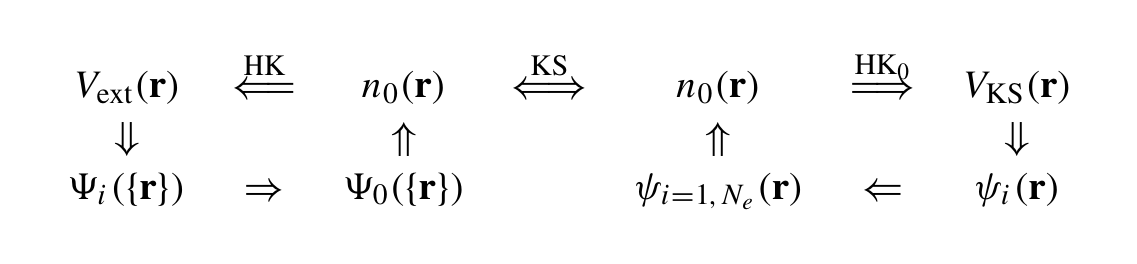
\includegraphics[width=0.8\linewidth]{corres.png}
	\caption{Correspondence relations in DFT}
	\label{fig:hk-relations}
\end{figure}

Figure \ref{fig:hk-relations} summarizes the logical flow of DFT. Given $v_{ext}(\mathbf{r})$, the many-body Schr\"odinger equation determines the eigenstates $\Psi_i(\{\mathbf{r}\})$, which include the ground state $\Psi_0$. The ground-state density is
$$n_0(\mathbf{r})=N\int d\mathbf{r}_2\cdots d\mathbf{r}_N|\Psi_0(\mathbf{r},\mathbf{r}_2,\ldots,\mathbf{r}_N)|^2$$
The non-trivial part is the reverse map $n_0(\mathbf{r})\to v_{ext}(\mathbf{r})$, which is the Hohenberg--Kohn theorem.

\begin{itemize}
	\item Theorem 1. For a non-degenerate ground state, $v_{ext}(\mathbf{r})$ and $n_0(\mathbf{r})$ have a one-to-one correspondence (up to an additive constant in $v_{ext}$). Consequently, $n_0(\mathbf{r})$ determines the full Hamiltonian and all ground-state properties.
	\item Theorem 2. There exists a universal functional $F[n]$ such that the total energy for a given external potential is
	      $$E_v[n]=F[n]+\int d\mathbf{r}\, v_{ext}(\mathbf{r})n(\mathbf{r})$$
	      and the ground-state density minimizes $E_v[n]$.
\end{itemize}

A sketch of the first theorem is by contradiction. Suppose two distinct external potentials $v_{ext}^1$ and $v_{ext}^2$ (not differing by a constant) yield the same ground-state density $n_0(\mathbf{r})$, with ground states $|\Psi^1\rangle$ and $|\Psi^2\rangle$. The variational principle gives
$$E^1<\langle\Psi^2|H^1|\Psi^2\rangle=E^2+\int d\mathbf{r}\,\bigl(v_{ext}^1(\mathbf{r})-v_{ext}^2(\mathbf{r})\bigr)n_0(\mathbf{r})$$
and, by symmetry,
$$E^2<\langle\Psi^1|H^2|\Psi^1\rangle=E^1+\int d\mathbf{r}\,\bigl(v_{ext}^2(\mathbf{r})-v_{ext}^1(\mathbf{r})\bigr)n_0(\mathbf{r})$$
Adding the two inequalities gives a contradiction, so the densities cannot be the same.

\subsection*{Levy--Lieb Functional}
Not every physically admissible density is the ground-state density of some external potential (v-representable), but any antisymmetric $N$-electron wavefunction defines a density (N-representable). Levy and Lieb defined the constrained-search functional
$$F_{LL}[n]=\min_{\Psi\to n}\langle\Psi|T+W|\Psi\rangle$$
which is valid for all N-representable densities and coincides with $F[n]$ on v-representable ones. The ground-state energy follows from minimizing
$$E_v[n]=F_{LL}[n]+\int d\mathbf{r}\,v_{ext}(\mathbf{r})n(\mathbf{r})$$

\subsection*{Kohn--Sham Equation}
Kohn and Sham introduced a non-interacting reference system that reproduces the interacting ground-state density (the non-interacting v-representability assumption). The density is written in terms of single-particle orbitals,
$$n(\mathbf{r})=\sum_i|\psi_i(\mathbf{r})|^2$$
and the Kohn--Sham energy functional is
$$E_{KS}[n]=T_s[n]+\int d\mathbf{r}\,v_{ext}(\mathbf{r})n(\mathbf{r})+E_H[n]+E_{XC}[n]$$
Here $T_s[n]$ is the kinetic energy of the non-interacting system,
$$T_s[n]=-\frac{1}{2}\sum_i\int d\mathbf{r}\,\psi_i^*(\mathbf{r})\nabla^2\psi_i(\mathbf{r})$$
and
$$E_H[n]=\frac{1}{2}\int d\mathbf{r}d\mathbf{r'}\frac{n(\mathbf{r})n(\mathbf{r'})}{|\mathbf{r}-\mathbf{r'}|}$$
The exchange-correlation functional collects all remaining many-body effects,
\begin{equation}
	E_{XC}[n]=F[n]-T_s[n]-E_H[n]\label{excdef}
\end{equation}
Minimizing $E_{KS}[n]$ with respect to $\psi_i^*(\mathbf{r})$ (with orthonormality constraints) yields the Kohn--Sham equations
\begin{equation}
	\left(-\frac{1}{2}\nabla^2+v_{ext}(\mathbf{r})+v_H(\mathbf{r})+v_{XC}(\mathbf{r})\right)\psi_i(\mathbf{r})=\epsilon_i\psi_i(\mathbf{r})\label{kse}
\end{equation}
where
$$v_H(\mathbf{r})=\frac{\delta E_H}{\delta n(\mathbf{r})}=\int d\mathbf{r'}\frac{n(\mathbf{r'})}{|\mathbf{r}-\mathbf{r'}|},\quad
	v_{XC}(\mathbf{r})=\frac{\delta E_{XC}}{\delta n(\mathbf{r})}$$
In practice, the Kohn--Sham equations are solved self-consistently:
\begin{enumerate}
	\item Take an initial guess of $n(\mathbf{r})$
	\item Construct $v_{KS}(\mathbf{r})=v_{ext}(\mathbf{r})+v_H(\mathbf{r})+v_{XC}(\mathbf{r})$
	\item Solve the Kohn--Sham equation for $\{\psi_i\}$
	\item Update $n(\mathbf{r})=\sum_i|\psi_i(\mathbf{r})|^2$
	\item If the new density differs from the old one, iterate from 2
	\item Compute the total energy from the functional $E_{KS}[n]$ (the eigenvalue sum alone double-counts interactions)
\end{enumerate}
\begin{figure}[ht]
	\centering
	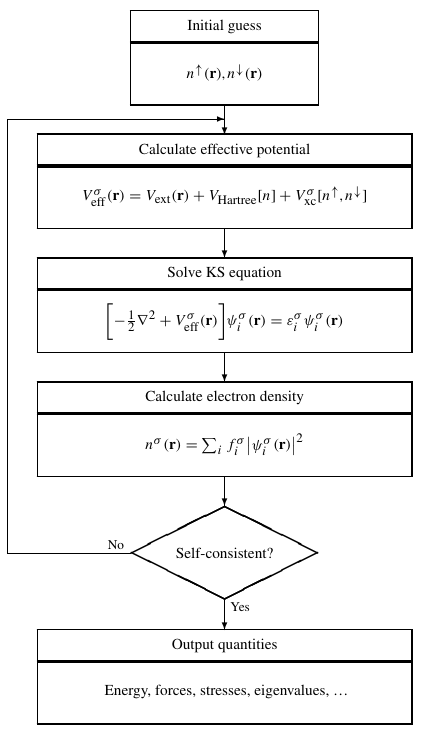
\includegraphics[width=0.5\linewidth]{flow.png}
	\caption{Solving Kohn--Sham equations self-consistently}
	\label{fig:ks-scf}
\end{figure}
After obtaining the converged density, one can evaluate material properties as derivatives of the total energy. But let's first look into popular guesses for $E_{XC}[n]$.
\subsection*{Functional form of $E_{XC}[n]$}
The Kohn--Sham equations are independent particle equations; all many-body effects are contained in $E_{XC}[n]$ if it were exact. But some reasonable guesses of $E_{XC}[n]$ were both accurate and computationally accessible, bringing success to DFT.\\
$E_{XC}[n]$ is usually expressed in the form of
$$E_{XC}[n]=\int d\mathbf{r}n(\mathbf{r})\varepsilon_{XC}([n],\mathbf{r})$$
where $\varepsilon_{XC}$ is the single electron energy that depends on $[n]$ and $\mathbf{r}$.\\
In the Local Density Approximation (LDA), materials are assumed to be homogeneous enough that exchange-correlation takes effect only locally.
$$E^{LDA}_{XC}[n]=\int d\mathbf{r} n(\mathbf{r})\varepsilon_{XC}^{hom}(n(\mathbf{r}))$$
$\varepsilon_{XC}^{hom}$ is the exchange-correlation energy per electron of the homogeneous electron gas (a free electron gas in a positive background for charge neutrality). In the homogeneous electron gas, exchange and correlation effects are separable, with the exchange energy per electron given by
$$\varepsilon_X(n)=-\frac{3}{4}\left(\frac{3}{\pi}\right)^{1/3}n^{1/3}$$\\
The Generalized Gradient Approximation (GGA) attempts an expression of $n$ including its first derivative,
$$E^{GGA}_{XC}[n]=\int d\mathbf{r} n(\mathbf{r})\varepsilon_{XC}^{hom}F_{XC}(n(\mathbf{r}),|\nabla n(\mathbf{r})|)$$
where $F_{XC}$ is the GGA functional that we have to guess the form of. \\
GGAs, as they are extensions of LDA, may seem to yield more accurate results. However, real materials' electronic structure is very subtle. Just by adding the first order derivative of $n$ doesn't do the magic trick. LDA and GGA are just the simplest form of functionals to write down. There are functionals with increasing levels of complexity to capture more completely the XC nature of electrons. Examples are Meta-GGAs that incorporate electron kinetic energy into the functional, or hybrid functionals and pseudopotentials (a formalism on its own to account for core-electron interaction), and functionals of response functions to better capture the band gap problem. Some functionals are even machine-learned to fit experimental data. All these different functionals are a different book on its own, giving vast diversity in DFT application and research.\\
What will the knowledge of $E_g$ enable us to do, after an educated guess of $E_{XC}[n]$? Many physical quantities are derivatives of $E$, such as the heat capacity $C=\frac{\partial E}{\partial T}$, Polarizability $\alpha_{ij}=\frac{\partial^2 E}{\partial\mathcal{E}_i\partial\mathcal{E}_j}$, Elasticity Tensor $C_{ijkl}=\frac{\partial^2 E}{\partial\epsilon_{ij}\partial\epsilon_{kl}}$, magnetic susceptibility $\chi_{ij}=\frac{\partial^2 E}{\partial B_i \partial B_j}$ and many others. Further applications include equilibrium structure and bond length calculation (simply by calculating $E_g$s of different configurations), vibrational modes and phonons, the band structure itself, optical spectra, phase diagram, etc. With its wide spectrum of use, DFT successfully brought quantum physics to the level of materials science.

\section*{Quaiparticles}
\subsection*{Landau Fermi Liquid Theory}
Our derivation of the band structure and density functional theory was based on an independent particle approximation. Particles are subject to an 'average' potential created by others which pairwise interactions were accounted for. When this pairwise interaction is significant, our scheme produces inexact results. A band metal may actually turn out as a Mott Insulator, other exotic behaviors that weren't predicted occurs. Yet in other cases, independent particle approximation yields accurate result for an oversimplified model. Landau's Fermi liquid theory (LFLT) is a phenomenological justification for such an assumption.\\
Consider a multi electronic system. This time, we will allow the number of electron in the system to vary, by introducing the grand Hamiltonian
$$H=T+\lambda V-\mu N$$
$T$ is the kinetic energy of electrons, $V$ is the electron-electron interaction and $N$ is the total number of electrons which is counted by $N=\sum_{\mathbf{k}}n_{\mathbf{k}}$. $n_{\mathbf{k}}$ is the occupation number of the electron at state $\mathbf{k}$ in the $\mathbf{k}$ space. By ignoring thermal fluctuation induced Fermi-Dirac occupation factor, $n_{\mathbf{k}}$ will take $0$ or $1$ as its value. $\mu$ is the chemical potential, related again to the occupation in $\mathbf{k}$ space. ($\mu=\mathbf{k}_F$ in the free electron ground state). $\lambda$ is the parameter varying from $0$ to $1$, determining strength of the 'perturbing' electron-electron interaction.\\
Consider first the $\lambda=0$ case, which is essentially the free electron gas. When using $N=\sum_{\mathbf{k}}$
$$H=\sum_{\mathbf{k}}\Biggl(\frac{\hbar^2\mathbf{k}^2}{2m}-\mu\Biggr)n_{\mathbf{k}}=\sum_{\mathbf{k}}\epsilon_{\mathbf{k}}n_{\mathbf{k}}$$
$\epsilon_{\mathbf{k}}=\frac{\hbar^2\mathbf{k}^2}{2m}-\mu$ is the energy of each 'independent' electron measured from the chemical potential $\mu$. In the ground state occupancy factor $n_{\mathbf{k}}^{0}$is as follows
$$n_{\mathbf{k}}^{0}=
	\begin{cases}
		1\hspace{5mm}(\frac{\hbar^2\mathbf{k}^2}{2m}\leq\mu) \\
		0\hspace{5mm}(\frac{\hbar^2\mathbf{k}^2}{2m}\geq\mu)
	\end{cases}$$
The excitation number $\delta n_{\mathbf{k}}=n_{\mathbf{k}}-n_{\mathbf{k}}^{0}=0$\\
The gist of Fermi liquid theory is to adiabatically(slowly) turn on the interaction $V$. The system than has no choice but to excite our of the Fermi surface.
$$\delta _{\mathbf{k}}
	\begin{cases}
		0,1\hspace{6mm}\mathbf{k}>\mathbf{k}_F \\
		0.-1\hspace{2mm}\mathbf{k}<\mathbf{k}_F
	\end{cases}
$$
Consider a cases when a single electron has been excited, leaving a 'hole' in the Fermi sphere. The excitation energy $\epsilon_{\mathbf{k}}$ is
$$\epsilon_{\mathbf{k}}=\frac{\hbar^2|\mathbf{k}-\mathbf{k}_F|^2}{2m}>0$$
The cost of removing an electron from the system $\mu$ is the increase of energy in the system by 'decreasing' the number of electrons. In the case of excitations near the Fermi surface,
$$\epsilon_{\mathbf{k}}=\frac{\hbar^2|\mathbf{k}-\mathbf{k}_F|^2}{2m}\sim\hbar\mathbf{v}_F|\mathbf{k-\mathbf{k_F}}|$$
Adding or removing an electron or a hole near the Fermi surface has a well defined dispersion($\mathbf{k}\to\epsilon$) relation and they are the smallest quanta of all other possible excitations. We call such excitation a low-energy excitation.\\
Suppose $\lambda$ is turned on to its maximum, resulting in a certain excited state. Is it possible to follow adiabatically(step by step) well defined single electron-hole excitation from free electron gas to any strong-excited state? It is easy to see such connection is not possible due to degeneracy. Even for a low energy excitation $\mathbf{k}_0>\mathbf{k}_F$, it is possible to fine many two electron - one hole excitation, $\mathbf{k}_1,\mathbf{k}_3>\mathbf{k}_F$, $\mathbf{k}_2<\mathbf{k}_F$ that is degenerate with a single excitation by the following simple condition.
$$\mathbf{k}_0=\mathbf{k}_1+\mathbf{k}_3-\mathbf{k}_2, \hspace{5mm}|\mathbf{k}_0|=|\mathbf{k}_1|+|\mathbf{k}_3|-|\mathbf{k}_2|$$
Landau's idea is that for the case of low energy excitations, degeneracy wouldn't be significant and adiabaticity will hold approximately, even when interaction is noticeable. That is, for the case of
$$\delta\mathbf{k}_0\mathbf{k}_0-\mathbf{k}_F<<\mathbf{k}_F, \hspace{5mm}\epsilon_{\mathbf{k}}\sim\hbar v_{F}\delta\mathbf{k}_0$$
adiabaticity will hold, with an argument due to the energy-time uncertainty $\Delta E\Delta t\geq\frac{\hbar}{2}$.\\
From Fermi's golden rule, the transition scattering time $\tau_{\mathbf{k}_0}$ goes like
$$\tau_{\mathbf{k}_0}\propto\delta \mathbf{k}_0^{-2}$$
So the energy-time uncertainty yields
$$\delta\epsilon_{\mathbf{k}_0}\propto\delta\mathbf{k}_0^2$$
For the low energy excitation which has small values for $\delta\mathbf{k}_0$, would have the following inequality
$$\delta\epsilon_{\mathbf{k}_0}<<\epsilon_{\mathbf{k}_0}$$
In the case of low energy excitation, uncertainty in excitation energy is much smaller than the excited energy. In simpler words, in low energy excitation adiabatic connection from non-interacting ground state is satisfied because there is not much state elsewhere in $\mathbf{k}$ space for the excited state to be. Good news is, condensed matter is almost always probed in the realm of low energy(we can never really strictly look in to the true ground state due to thermal fluctuation and imperfections, so low energy excitation is our main ground).\\
These low energy excitations are called quasiparticles/holes, in this previous case, quasielectrons excited out of the 'vacuum' of ground state free electron gas that we know perfectly of. The characteristics of these quasiparticles and their corresponding vacuums are central to understanding the property of materials. Landau's Fermi liquid theory occasionally fails when in the progress of turning on the interaction, quantum phase transition occurs. In such cases, many exotic behaviors will be observed each requiring a different formalism to explain. Many materials that can be safely excited from their ground state are called 'normal' and our formalisms of Bloch theorem and LFLT safely applies for normal materials.
\subsection*{Quasielectron}
Quasielectrons are electrons that have excited from the 'vacuum' of free electrons gas to a state near the Fermi surface. Quasielectrons and holes have many peculiar physical quantities, most notably the effective mass $m^*_{ij}$.\\
We derive effective mass tensor $m^*_{ij}$ first from the semiclassical equation(yes, the mass is tensor valued, also the asterisk superscript will be used to denoted effective variables). First, form a tensor-version of Newton's equation of motion.
$$\sum_j\Biggl(\frac{1}{m^*}\Biggr)_{ij}\mathbf{F}^*_{ij}=\mathbf{a}_{i}^{*}$$
Then from one of the semiclassical equation \eqref{semione},
$$\mathbf{a}_{i}^{*}=\frac{d\mathbf{v}_{i}^{*}}{dt}=\frac{1}{\hbar}\frac{d}{dt}\frac{\partial \epsilon_n(\mathbf{k})}{\partial\mathbf{k}_i}=\frac{1}{\hbar}\sum_j\frac{\partial^2 \epsilon_n(\mathbf{k})}{\partial\mathbf{k}_i\partial\mathbf{k}_j}\frac{d\mathbf{k}_j}{dt}$$
And the second semiclassical equation \eqref{semitwo}
$$\mathbf{a}_{i}^{*}=\sum_j\frac{1}{\hbar^2}\frac{\partial^2 \epsilon_n(\mathbf{k})}{\partial\mathbf{k}_i\partial\mathbf{k}_j}\mathbf{F}_j^*$$
The effective mass tensor is finally given by
$$\frac{1}{m_{ij}^{*}}=\frac{1}{\hbar}\frac{\partial^2 \epsilon_n(\mathbf{k})}{\partial\mathbf{k}_i\partial\mathbf{k}_j}$$
We see that $m_{ij}^{*}$ is determined by the curvature of $\epsilon_n(\mathbf{k})$. The 'stronger' the curvature, smaller is $m^*$\\
An alternative approach to $m^*$ is possible to relieve ourselves of the single-band assumption of semiclassical equation. From \eqref{eigenvalueeqwithbandstructure},
$$\Biggl(\frac{(\mathbf{p}+\hbar\mathbf{k})^2}{2m}+V(\mathbf{r})\Biggr)u_{n\mathbf{k}}(\mathbf{r})=\epsilon_n(\mathbf{k})u_{n\mathbf{k}}(\mathbf{r})$$
We that we know the value of $\epsilon_n(\mathbf{k})$ at $\mathbf{k}_0$, and are trying to extrapolate $\epsilon_n(\mathbf{k}')$ where $\mathbf{k}'$ is in the vicinity of $\mathbf{k}_0$, $\mathbf{k}'=\mathbf{k}_0+\delta\mathbf{k}$,
$$\Biggl(\frac{(\mathbf{p}+\hbar\mathbf{k}')^2}{2m}+V(\mathbf{r})\Biggr)u_{n\mathbf{k}'}(\mathbf{r}')=\epsilon_n(\mathbf{k}')u_{n\mathbf{k}'}(\mathbf{r}')$$
$$\Biggl(\frac{(\mathbf{p}+\hbar\mathbf{k}_0)^2}{2m}+V(\mathbf{r})+\frac{\hbar\delta\mathbf{k}\cdot(\mathbf{p}+\hbar\mathbf{k}_0)}{m}+\frac{\hbar^2\delta\mathbf{k}^2}{2m}\Biggr)u_{n\mathbf{k}'}(\mathbf{r}')=\epsilon_{n\mathbf{k}'}u_{n\mathbf{k}'}(\mathbf{r}')$$
We take the third term in the parentheses, $\hbar\delta\mathbf{k}\cdot(\mathbf{p}+\hbar\mathbf{k}_0)/m$ as the perturbation, which we call the $\mathbf{k}\cdot\mathbf{p}$ perturbation method. Upon second order degenerate perturbation theory,
\begin{multline}
	\epsilon_{n}(\mathbf{k}_0+\delta\mathbf{k})=\frac{\hbar^2\delta\mathbf{k}^2}{2m}+\epsilon_{n}(\mathbf{k}_0)+\frac{\langle u_{n\mathbf{k}_0}|\hbar\delta\mathbf{k}\cdot(\mathbf{p}+\hbar\mathbf{k}_0)|u_{n\mathbf{k}_0}\rangle}{m}+\\
	\sum_{n\neq n'}\frac{|\langle u_{n\mathbf{k}_0}|\hbar\delta\mathbf{k}\cdot(\mathbf{p+\hbar\mathbf{k_0}})|u_{n'\mathbf{k}_0}\rangle|^2}{m(\epsilon_{n}(\mathbf{k}_0)-\epsilon_{n'}(\mathbf{k}_0))}
\end{multline}
Comparing this result to the simple second order expansion around $\mathbf{k}_0$
$$\epsilon_n(\mathbf{k}_0+\delta\mathbf{k})=\epsilon_n(\mathbf{k}_0)+=\sum_i\frac{\partial\epsilon_n(\mathbf{k}_0)}{\partial\mathbf{k}_i}\mathbf{k}_i+\sum_{i\neq j}\frac{\partial\epsilon_n(\mathbf{k}_0)}{\partial\mathbf{k}_i\partial\mathbf{k}_j}\mathbf{k}_i\mathbf{k}_j$$
The first order term yields a familiar result to the semiclassical equation
\begin{multline*}
	\frac{\hbar}{m}\langle u_{n\mathbf{k}_0}|\mathbf{p}_i+\hbar\mathbf{k}_i|u_{n\mathbf{k}_0}\rangle=\frac{\hbar}{m}\langle\psi_{n\mathbf{k}_i}(\mathbf{r})|\mathbf{p}_i|\psi_{n\mathbf{k}_i}(\mathbf{r})\rangle=
	\frac{\hbar}{m}\mathbf{v}_{i}^{*}=\frac{\partial\epsilon_n(\mathbf{k}_0)}{\partial\mathbf{k}_i}
\end{multline*}
Where we have shown an alternate definition of effective velocity\\
$\mathbf{v}_{i}^*=\langle\psi_{n\mathbf{k}}(\mathbf{r})|\mathbf{p}_i|\psi_{n\mathbf{k}(\mathbf{r})}\rangle/m$.
Comparing the second order term,
$$\sum_{i\neq j}\frac{\partial\epsilon_n(\mathbf{k}_0)}{\partial\mathbf{k}_i\partial\mathbf{k}_j}\mathbf{k}_i\mathbf{k}_j=\sum_{n\neq n'}\frac{|\langle u_{n\mathbf{k}_0}|\hbar\delta\mathbf{k}\cdot(\mathbf{p+\hbar\mathbf{k_0}})|u_{n'\mathbf{k}_0}\rangle|^2}{m(\epsilon_{n}(\mathbf{k}_0)-\epsilon_{n'}(\mathbf{k}_0))}$$
yields a complex form,
$$\frac{m}{(m^*_{n})_{ij}}=\delta_{ij}+\sum_{n\neq n'}f_{nn'}^{ij}$$
\begin{multline*}
	f_{nn'}^{ij}=\frac{\langle\psi_{n\mathbf{k}_0(\mathbf{r})}|\mathbf{p}_i|\psi_{n\mathbf{k}_0(\mathbf{r})}\rangle\langle\psi_{n\mathbf{k}_0(\mathbf{r})}|\mathbf{p}_j|\psi_{n'\mathbf{k}_0(\mathbf{r})}\rangle}{m(\epsilon_n(\mathbf{k}_0)-\epsilon_{n'}(\mathbf{k}_0))}+\\
	\frac{\langle\psi_{n'\mathbf{k}_0(\mathbf{r})}|\mathbf{p}_j|\psi_{n\mathbf{k}_0(\mathbf{r})}\rangle\langle\psi_{n\mathbf{k}_0(\mathbf{r})}|\mathbf{p}_i|\psi_{n'\mathbf{k}_0(\mathbf{r})}\rangle}{m(\epsilon_n(\mathbf{k}_0)-\epsilon_{n'}(\mathbf{k}_0))}
\end{multline*}
The f-function and the corresponding $m^*$ depends on the harmonic contribution of $\epsilon_n(\mathbf{k}_0)$ and also the band gap. Consider a quasielectron-hole pair at the band edge where band 1 is the valence band, band 2 a conduction band. If the band curvature and $\mathbf{p}$ is isotopic, $m_1^*$ and $m_2^*$ reduces to
$$\frac{m}{m^*}=1\pm\frac{2}{m}\frac{|p|^2}{E_g}$$
Here, $E_g$ is the band gap, $+$ sign for $m_2^*$, $-$ sign for $m_1^*$. From this simplified model, smaller gap indicates smaller $m^*$. When $E_g$ is small enough, $m_1^*$ may even take negative values. %consult kittel%
\subsection*{Phonon}
Phonons are collective excitation of lattice vibration model. In the quasiparticle scheme, their vacuum is the perfect lattice and phonons are vibrational excitations out of it. Thermal vibrations or external probes cause vibration at one side of a lattice which then disperses throughout the entire lattice. Unlike quasielectrons, it is hard to imagine vibrations as particles. That is why they are referred to as 'collective excitations' which are bosons unlike quasielectrons(fermions). But in the quantum formulation of Phonons, we will mathematically formulate them into the 'scheme' of particles.
\subsection*{Classical vibration of harmonic crystal}
We first consider the simplest case of 1D monatomic chain.\\
In the 1D monatomic chain, a total of $N$  atoms are located at $na$, $(n+1)a$, $(n+2)a\cdots$ with $a$ as the lattice parameter. These are the equilibrium position of these atoms and non-equilibrium oscillations will be denoted with respect to the equilibrium position, like $u_{na}$\\
We can approximate that each atom experiences a harmonic potential, essentially thinking of them as connected springs with we set the spring constant as $q$ and each atomic mass $m$. The amplitude of oscillation should be minute compared to lattice parameter $a$ for the ease of taylor expansion. The potential the atoms experience are
$$V^{harm}=\frac{1}{2}k\sum_n(u_{na}-u_{(n+1)a})^2$$
So their equation of motion are
$$-\frac{\partial V^{harm}}{\partial u_{na}}=m\frac{d^2 u_{na}}{dt^2}=-k(2u_{na}-u_{(n+1)a}-u_{(n-1)a})$$
we search for solutions to this equation under the periodic boundary condition $u_0=u_{Na}$ by making an educated guess in the form of $u_{na}(t)=e^{i(qna-\omega t)}$.\\
This boundary conditions yields $q=\frac{2\pi n}{Na}$ where $n$ is a non-negative integer. Substituting the ansatz in to the equation of motion yields
$$-m\omega^2e^{i(qna-\omega t)}=-2k(1-cos(qa))e^{i(qna-\omega t)}$$
The dispersion relation, $\omega(k)$ is
$$\omega(k)=2\sqrt{\frac{k}{m}}|sin(qa/2)|$$
Notice the linear relationship, $\omega(k)\sim a\sqrt{k/m}|q|$ near $k=0$ and the vanishing group velocity $v_g=\frac{\partial \omega}{\partial q}$ at $q=\pm\frac{\pi}{a}$. Evaluation outside of $q=\pm\frac{\pi}{a}$ is redundant, just as it was with the case of Brillouin zone of Bloch state. Such linear relation near $q=0$ (providing a justification for Debye approximation of heat capacity) and the 'gapless' excitation $\omega(0)=0$, vanishing $v_g$ at the 'Phonon' edge is a common trait among many other collective excitations.\\
Next, consider the case of two atoms per primitive cell, with atom 1 at the position $na$, $(n+1)a$, $(n+2)a\cdots$ and atom 2 positioned at $na+d$, $(n+1)a+d$, $(n+2)a+d\cdots$. The spring constant is different for each connection of atom, $k$ for $1-2$ connection and $g$ for $2-1$ connection. With the same procedure, we arrive at the potential
$$V^{harm}=\frac{k}{2}\sum_n(u^1_{na}-u^2_{na})^2+\frac{g}{2}\sum_n(u^2_{na}-u^2_{(n-1)a})^2$$
The superscript at $u$ indicates which atom's oscillation it is describing. $V^{harm}$ further gives us the equation of motions, one for each type of atom
$$m\frac{d^2 u^1_{na}}{dt^2}=-\frac{\partial V^{harm}}{\partial u^1_{na}}=-k(u^1_{na}-u^2_{na})-g(u^1_{na}-u^2_{(n-1)a})$$
$$m\frac{d^2 u^2_{na}}{dt^2}=-\frac{\partial V^{harm}}{\partial u^2_{na}}=-k(u^2_{na}-u^1_{na})-g(u^2_{na}-u^1_{(n+1)a})$$
We will again substitute the solution form of
$$u^{1,2}_{na}=\epsilon_{1,2}e^{i(qna-\omega t)}$$
With $\epsilon_1$ and $\epsilon_2$ as the relative amplitude of vibration. Substitution and some calculations yield the dispersion relation $\omega(q)$
$$\omega(q)=\frac{k+g}{m}\pm\frac{1}{m}\sqrt{k^2+g^2+2kgcos(qa)}$$
and the relative amplitude
$$\frac{\epsilon_2}{\epsilon_1}=\mp\frac{k+ge^{iqa}}{|k+ge^{iqa}|}$$
There are two dispersion curves for this model. One that starts at $\omega(0)=0$ and showing a linear relation, just as the monatomic case is called the acoustic branch, another with $\omega(0)=\sqrt{(k+g)/m}$ is the optical branch. As in the case with monatomic case, $q$ is restricted in the first Brillouin zone, at $q=\pm\pi /a$. For the relative amplitude, $+$ sign is taken by the acoustic branch, $-$ by the optical branch. Near $q=0$, acoustic branch shows in-phase oscillations whereas optical branch shows out-of-phase oscillations.\\
Now let's consider of vibrational mode of 3D monatomic lattice. In order to extend the 'spring' analogy in 3D, simply taylor expand the lattice potential V upto second order. (We drop the $na$ notation and take index $j,k$ for atomic coordinates).
\begin{multline*}
	V(\mathbf{r}_1,\cdots,\mathbf{r}_{N})=V(\mathbf{R}_1,\cdots,\mathbf{R}_{N})+\sum_ju_j\cdot\nabla_j V\Biggl |_{\mathbf{r}=\mathbf{R}}\\
	+\frac{1}{2}\sum_{jk}(u_j\cdot\nabla_j)(u_k\cdot\nabla_k)V\Biggl|_{\mathbf{r}=\mathbf{R}}
\end{multline*}
We may ignore the first two terms from the equilibrium condition which allows us to rewrite 3D harmonic potential as
$V^{harm}=\frac{1}{2}\sum_{\mathbf{R}\mathbf{R}'}\sum_{jk}u_j(\mathbf{R})D_{jk}(\mathbf{R}-\mathbf{R}')u_k(\mathbf{R}')$
with $D_{jk}=\frac{\partial}{\partial u_j}\frac{\partial}{\partial u_k}V$
This dynamical matrix has the following property,
$$D_{jk}(\mathbf{R}-\mathbf{R}')=D_{kj}(\mathbf{R}'-\mathbf{R})$$
$$D_{jk}(\mathbf{R}-\mathbf{R}')=D_{jk}(\mathbf{R}'-\mathbf{R})$$
$$\sum_{\mathbf{R}}D_{jk}(\mathbf{R})=0$$
These properties each comes the the fact that 1. partial derivatives commute, 2. the lattice has inversion symmetry, 3. displacement of all atoms do nothing. The equation of motion is now
$$m\frac{d^2u_j(\mathbf{R})}{dt^2}=-\frac{\partial V^{harm}}{\partial u_j(\mathbf{R})}=-\sum_{\mathbf{R}'k}D_{jk}(\mathbf{R}-\mathbf{R}')u_k(\mathbf{R}')$$
We again seek solutions in the form of plane wave
$$u(q,\mathbf{R},t)=\epsilon(\mathbf{q})e^{i(\mathbf{q}\cdot \mathbf{R}-\omega t)}$$
$\epsilon(\mathbf{q})$ is now the polarization vector. Applying the periodic boundary condition $u(R_i+n_ia_i)=u(R_i)$ will again restrict $\mathbf{q}$ inside the first Brillouin zone. Substituting the solution again,
$$-m\omega^2\epsilon(\mathbf{q})=-\sum_{\mathbf{R'}k}D_{jk}(\mathbf{R}-\mathbf{R'})\epsilon(\mathbf{q})e^{i\mathbf{q}\cdot(\mathbf{R}-\mathbf{R'})}$$
Fourier transforming $D_{jk}$, $\sum_\mathbf{R}D_{jk}(\mathbf{R})e^{-i\mathbf{q}\cdot\mathbf{R}}$ we obtain
$$m\omega^2\epsilon(\mathbf{q})=D(\mathbf{q})\epsilon(\mathbf{q})$$
Notice $D(0)=0$, just as it was the case acoustic branch of phonon. Further calculation will also show linearity of this acoustic branch. In the $\mathbf{q}\to0$ limit which is the long wavelength vibration, in a local observation atoms are just almost uniformly displaced, which is why it costs so little energy. Further calculation for $\omega(\mathbf{q})$ in a 3D lattice with $n$ atoms per primitive cell will yield 3 acoustic branches and $3(n-1)$ optical branches.
\subsection*{Quantum formulation of phonon}
We have looked in to normal modes of lattice vibrations, but how do we view these modes as particles? This is done by the creation and annihilation operator method used for the quantum harmonic oscillator.\\
Consider a set of decoupled oscillators each located at $R_i$. Their Hamiltonian is
$$H=\sum_i\frac{p_i^2}{2m}+\frac{1}{2}ku_{i}^{2}$$
When all the oscillators are at the ground state, such state is denoted $|0\rangle$. We excite the $j$th oscillator with the 'creation' operator $a_j^{\dagger}$
$$|1_j\rangle=a_{j}^{\dagger}|0\rangle$$
and its hermitian conjugate $a_j$ is the annihilation operator,
$$|0\rangle=a_j|1_j\rangle$$
The specific form of these operator is
$$a_{j}^{\dagger}=\sqrt{\frac{m\Omega}{2\hbar}}u_j-i\sqrt{\frac{1}{2m\hbar\Omega}}p_j$$
with $\Omega=\sqrt{k/m}$. The creation and annihilation operators obey the following commutation relation,
$$[a_i,a_j]=0,\hspace{5mm}[a_i,a_{j}^{\dagger}]=\delta_{ij}$$
These are the bosonic commutation relations showing that our phonons are boson.\\
As was with many other cases, we want information in the momentum space, the Fourier transformed operator $a^{\dagger}(\mathbf{q})$ is given by
$$a^{\dagger}(\mathbf{q})=\frac{1}{N}\sum_je^{i\mathbf{q}\cdot\mathbf{R}_j}a_{j}^{\dagger}$$
$$[a(\mathbf{q}),a(\mathbf{q}')]=0,\hspace{5mm}[a(\mathbf{q}),a^{\dagger}(\mathbf{q}')]=\delta_{\mathbf{k},\mathbf{k'}}$$
$a^{\dagger}(\mathbf{q})$ creates a phonon with wave vector $\mathbf{q}$. In this momentum space operator, $H$ takes a familiar diagonal form
$$H=\sum_j\hbar\Omega(a^{\dagger}_ja_j+1/2)=\sum_{\mathbf{q}}\hbar\Omega(a^{\dagger}(\mathbf{q})a(\mathbf{q}+1/2)$$
For considering actual phonon rather than decoupled oscillators just substitute $\Omega\to\omega(\mathbf{q})$. The familiar zero-point vacuum energy $\frac{1}{2}\hbar\omega$ is also present in phonon. These phonon particles contribute greatly to various properties, notably the heat capacity or by interaction with other quasiparticles. \\
To wrap things up in the quasiparticle picture, the actual crystal is made of atoms and electrons with strong and significant interactions. But low energy excitations such as phonon is only weakly interacting. When inquiring the low energy property of these crystals, we only need to solve the simple effective Hamiltonian(such as the decoupled oscillator Hamiltonian) instead of the complex 'actual' Hamiltonian. There are many other examples of quasiparticles other than quasielectrons and phonons. Quasielectrons and phonons are just one of the many quasiparticles to be discussed. We might as well define as much as we want - granted that we know of its ground state perfectly. To mention a few, magnons are bosonic excitations of spin wave whilst plasmons are its analog with electronic charge density. Plasmon oscillation frequency, $\omega_p=\sqrt{4\pi ne^2/m_e}$ and its derivation is commonly shown in elementary textbooks. Another is exciton, bound state of quasielectron and hole, frequently observed in semiconductor and insulators. Polarons are quasiparticles that 'carry' lattice deformation in certain types of crystal structure. Cooper pairs are quasiparticles contributing to the BCS superconductivity. Photon, quanta of light may also be considered quasiparticles if they are seen as excitations of electromagnetic wave(though pushing the argument this far may blur the distinction of quasiparticle and particle).
\end{document}

